\chapter{Entwicklung eines technischen Objekts}
%TODO Einleitung: Idee
% explizite Bezug auf Ultimaker 2, andere Drucker liefern andere Ergebnisse

Dieses Kapitel handelt vom Entwerfen und Drucken eines technischen Objekts. Als Objekt wird hier exemplarisch ein Aufbewahrungssystem f�r einen Raspberry Pi gekoppelt mit einem \ac{USB}- Hub und einer  externen Festplatte entworfen. Dieses System soll m�glichst kompakt sein und als ein Block transportierbar sein.

Diese Arbeit bezieht sich h�ufig auf den ultimaker 2, der im vorhergehenden Kapitel \ref{chapter:techGr:ultimaker2} vorgestellt wird. In der Arbeit mit einem anderen Drucker k�nnen sich Vorgehensweise und Ergebnis deutlich unterscheiden.

Zuerst wird die Analyse der bestehenden Verwahrung beschrieben. Anschlie�end folgt eine Beschreibung des umzusetzenden Konzepts. Folgend wird ein Entwurf des Systems mit einem \ac{CAD}-Programm  und der Druck des Objekts beschrieben. Der darauffolgende Abschnitt besch�ftigt sich mit w�hrend dem Druck aufgetretenen Fehlern. Zuletzt folgt ein Fazit �ber die Eignung des ultimaker 2 zum Drucken von technischen Objekten.


%TODO Ist-Analyse
\newpage
\section{Ist-Analyse}
	\piccaption{Urspr�ngliches Stapelsystem}
	\parpic{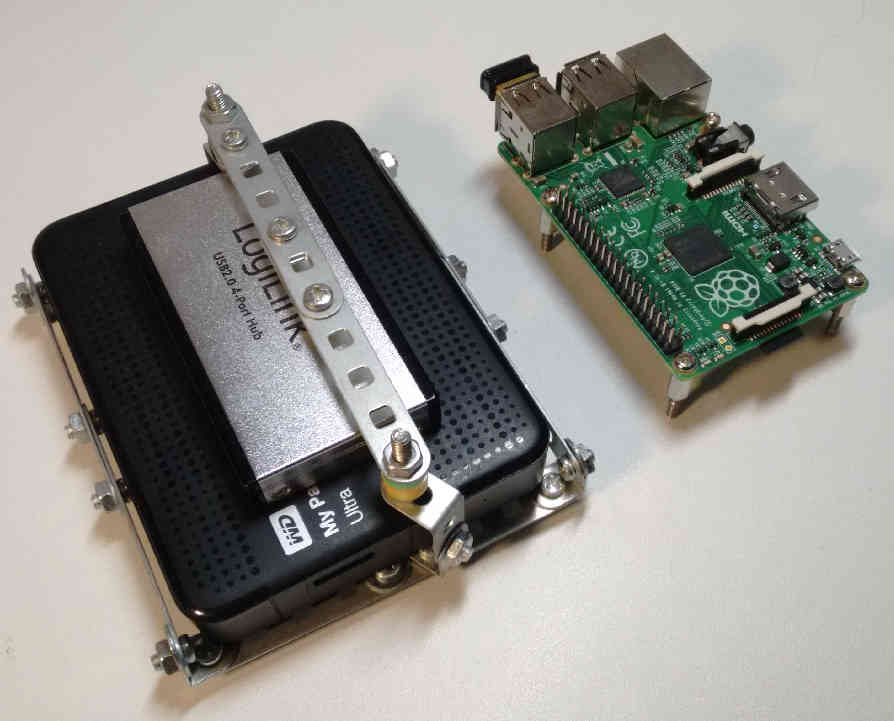
\includegraphics[width=.5\textwidth]{images/techObj/urspruenglicheHalterung02.jpg}}
	
	\picskip{0}
	
%TODO 
\section{Konzept: Modulare Boxen}
	Als Ersatz f�r den oben beschriebenen Rahmen soll ein modulares Stapelsystem dienen. Auf einer massiven Grundplatte werden Boxen gestapelt. Jede Box beinhaltet eine Komponente (Box, Hub oder Festplatte). Die Au�enma�e der Grundfl�chen der Boxen sind in Breite und L�nge immer gleich. Die Grundfl�che wird durch die gr��te zu befestigende Komponente, hier also die Festplatte, bestimmt. Der Innenraum einer Box ist an die jeweilige Komponente angepasst. Abh�ngig von der Komponente sind verschiedene Aussparungen in den Seitenw�nden der Boxen, durch die Kabel gef�hrt werden k�nnen. Im Aufbewahrungssystem werden die Boxen auf der Grundplatte gestapelt.\\
	Zwischen die Boxen werden Rahmen gelegt, die die Box zwischen Gewindestangen fixieren. Diese sind in der Grundplatte festgeschraubt. Dadurch ist das Stapelsystem im Ganzen stabilisiert und kann problemlos transportiert werden. \\
	Das System ist zudem einfach um neue Komponenten erweiterbar, sofern diese von der Grundfl�che her nicht gr��er sind als die Grundfl�che der Boxen. F�r neue Komponenten kann eine eigene Box mit den passenden Au�enma�en und angepasstem Innenraum und H�he entwickelt werden. Diese Box kann dann wie beschrieben mit Rahmen am System befestigt werden.



\section{Entwurf}
%Erw�hnen, dass Solid Edge verwendet

\section{Druck des Objekts}
% Wie w�re es ideal gewesen?, fertiges Objekt 
% Welche Parameter? --> spezifisch beim technischen Objekt
% Verlinkung zu Fehlern

\section{Aufgetretene Fehler}
% Bilder
% Fehleranalyse, [Ma�nahmen --> technische Grundlagen]

\section{Fazit: Eignung f�r technische Objekte}
% bezogen auf Ultimaker